\documentclass{report}
\usepackage[margin=1in, paperwidth=8.5in, paperheight=11in]{geometry}
%Math packages%
\usepackage{amsmath}
\usepackage{amsthm}
%Spacing%
\usepackage{setspace}
\onehalfspacing
%Lecture number%
\newcommand{\lectureNum}{5}
%Variables - Date and Course%
\newcommand{\curDate}{February 8, 2017}
\newcommand{\course}{MATH 239}
\newcommand{\instructor}{}
%Defining the example tag%
%\theoremstyle{definition}%
\newtheorem{ex}{Example}[section]
%Setting counter given the lecture number%
\setcounter{chapter}{\lectureNum{}}
%Package for drawing graphs%
\usepackage{tikz}
\usepackage{verbatim}
\usetikzlibrary{arrows}

\begin{document}
%Note title%
\begin{center}
\begin{Large}
\textsc{\course{} | Tutorial \lectureNum{}}
\end{Large}
\end{center} 
\noindent \textit{Bartosz Antczak} \hfill
\textit{\curDate{}}
\rule{\textwidth}{0.4pt}
% Actual Notes%
\subsection*{Kuratowski's Theorem}
\begin{center}
\textit{A graph G is not planar $\iff$ it has a subgraph that is a subdivision of either $K_5$ (the pentagram) or $K_{3,3}$}
\end{center}
We'll be looking at problem set 7.6 in the course notes:
\section*{Problem 1(d)}
%TODO include chart%
Prove whether or not this graph is planar:
\begin{figure}[ht]
\begin{center}
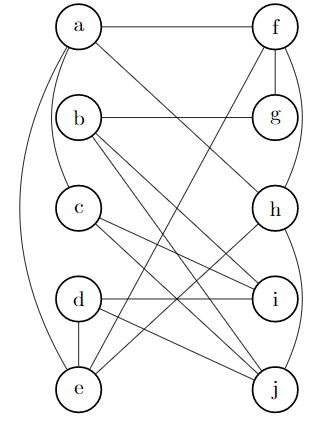
\includegraphics[scale=0.7]{graph1.jpg}
\end{center}
\end{figure}
There is no algorithm to determine this efficiently. We just have to play around with it. To prove that it's planar, we must show a planar embedding. If it's not planar, show that there exists a subdivision of either $K_5$ or $K_{3,3}$.\\In this case, this graph is \textit{not} planar.
\section*{Problem 8}
Consider the prime graph $B_n$, where the vertices of $B_n$ are $\{1, \cdots, n\}$, and there is an edge $uv$ if and only if $u+v$ is prime.
\begin{enumerate}
\item[a)] Prove that $B_8$ is planar\\
%TODO take a picture of the pretty graph I drew%
\end{enumerate}
%END%

\end{document}